%Copyright 2019 Christopher M. Jermaine (cmj4@rice.edu) and Risa B. Myers (rbm2@rice.edu)
%
%Licensed under the Apache License, Version 2.0 (the "License");
%you may not use this file except in compliance with the License.
%You may obtain a copy of the License at
%
%    https://www.apache.org/licenses/LICENSE-2.0
%
%Unless required by applicable law or agreed to in writing, software
%distributed under the License is distributed on an "AS IS" BASIS,
%WITHOUT WARRANTIES OR CONDITIONS OF ANY KIND, either express or implied.
%See the License for the specific language governing permissions and
%limitations under the License.
%===============================================================
\documentclass[aspectratio=169]{beamer}
\mode<presentation> 
{
\usetheme[noshadow, minimal,numbers,riceb,nonav]{Rice}
\usefonttheme[onlymath]{serif}
\setbeamercovered{transparent}
}
\useinnertheme{rectangles}
\usepackage{colortbl}

\usepackage[english]{babel}

\usepackage{mathptmx}
\usepackage{helvet}
\usepackage{courier}
\usepackage[T1]{fontenc}
\usepackage{trajan}
\usepackage{ textcomp }
\usepackage{amssymb}
\usepackage{tikz}   

%https://tex.stackexchange.com/questions/20740/symbols-for-outer-joins
\def\ojoin{\setbox0=\hbox{$\bowtie$}%
  \rule[-.02ex]{.25em}{.4pt}\llap{\rule[\ht0]{.25em}{.4pt}}}
\def\leftouterjoin{\mathbin{\ojoin\mkern-5.8mu\bowtie}}
\def\rightouterjoin{\mathbin{\bowtie\mkern-5.8mu\ojoin}}
\def\fullouterjoin{\mathbin{\ojoin\mkern-5.8mu\bowtie\mkern-5.8mu\ojoin}}


\usepackage{listings}

\newenvironment{noindentitemize}
{ \begin{itemize}
 \setlength{\itemsep}{1.5ex}
  \setlength{\parsep}{0pt}   
  \setlength{\parskip}{0pt}
 \addtolength{\leftskip}{-2em}
 }
{ \end{itemize} }

\newenvironment{noindentitemize2}
{ \begin{itemize}
  \setlength{\itemsep}{0ex}
  \setlength{\parskip}{0pt}
  \setlength{\parsep}{0pt}   
  \addtolength{\leftskip}{-2em}  }
{ \end{itemize} }

\lstnewenvironment{SQL}
  {\lstset{
        aboveskip=5pt,
        belowskip=5pt,
        escapechar=!,
        mathescape=true,
        upquote=true,
        language=SQL,
        basicstyle=\linespread{0.94}\ttfamily\footnotesize,
        morekeywords={PRINT, CURSOR, OPEN, FETCH, CLOSE, DECLARE, BEGIN, END, PROCEDURE, FOR, EACH, WITH, PARTITION, TEST, WHETHER, PROBABILITY, OUT,LOOP,IF,CONTINUE, HANDLER,CALL, FUNCTION, RETURNS, LANGUAGE,BODY,RETURN, ROUND,
        EXIT, TEXT, REFCURSOR, QUOTE_LITERAL, DELIMITER,CONCAT,FOUND,LEAVE, IF},
        deletekeywords={VALUE, PRIOR},
        showstringspaces=true}
        \vspace{0pt}%
        \noindent\minipage{0.6\textwidth}}
  {\endminipage\vspace{0pt}}

\lstnewenvironment{SQLtiny}
  {\lstset{
        aboveskip=5pt,
        belowskip=5pt,
        escapechar=!,
        mathescape=true,
        upquote=true,
        language=SQL,
        basicstyle=\linespread{0.94}\ttfamily\tiny,
        morekeywords={PRINT, CURSOR, OPEN, FETCH, CLOSE, DECLARE, BEGIN, END, PROCEDURE, FOR, EACH, WITH, PARTITION, TEST, WHETHER, PROBABILITY, OUT,LOOP,IF,CONTINUE, HANDLER,CALL, FUNCTION, RETURNS, LANGUAGE,BODY,RETURN,
        EXIT, TEXT, REFCURSOR, QUOTE_LITERAL, DELIMITER,CONCAT,FOUND,LEAVE, IF},
        deletekeywords={VALUE, PRIOR},
        showstringspaces=true}
        \vspace{0pt}%
        \noindent\minipage{0.47\textwidth}}
  {\endminipage\vspace{0pt}}
  
\newcommand{\AS}{\texttt{AS}} 
\newcommand{\SELECT}{\texttt{SELECT}} 
\newcommand{\WHERE}{\texttt{WHERE}} 
\newcommand{\ALL}{\texttt{ALL}} 
\newcommand{\UNION}{\texttt{UNION}} 
\newcommand{\EXCEPT}{\texttt{EXCEPT}} 
\newcommand{\LIKES}{\textrm{LIKES}} 
\newcommand{\FREQUENTS}{\textrm{FREQUENTS}} 
\newcommand{\SERVES}{\textrm{SERVES}} 
\newcommand{\CAFE}{\textrm{CAFE}} 
\newcommand{\COFFEE}{\textrm{COFFEE}} 
\newcommand{\DRINKER}{\textrm{DRINKER}} 
\newcommand{\CB}{\textrm{\textquotesingle{Cold} Brew\textquotesingle}} 
\newcommand{\CBGOOD}{\textrm{CBGOOD}} 
\newcommand{\ALLPEEPS}{\textrm{ALLPEEPS}} 
\newcommand{\ALLCOMBOS}{\textrm{ALLCOMBOS}} 
\newcommand{\NOGOODCOFFEE}{\textrm{NOGOODCOFFEE}} 

\setbeamerfont{block body}{size=\tiny}

%===============================================================%

\title[]
{Tools \& Models for Data Science}

\subtitle{SQL DDL and DML}

\author[]{Risa Myers}
\institute
{
  Rice University
}

\date[]{}


\begin{document}
\begin{frame}
 \titlepage
\end{frame}


%***********************************************************
\begin{frame}{DML \& DDL}

\begin{itemize}
\item Data Manipulation Language
\begin{itemize}
\item Data retrieval
\end{itemize}
\item Data Definition Language
\begin{itemize}
\item Used to specify the database schema
\item Generates a schema / data dictionary
\end{itemize}
\item Data Manipulation Language
\begin{itemize}
\item Data insertion
\item Data deletion
\item Data modification
\end{itemize}
\end{itemize}

\end{frame}

%***********************************************************
\begin{frame}{DDL}

\begin{itemize}
\item \texttt{CREATE TABLE}
\item \texttt{DROP TABLE}
\item \texttt{TRUNCATE TABLE}
\item \texttt{ALTER TABLE}
\end{itemize}

\end{frame}
%***********************************************************
\begin{frame}[fragile]{\texttt{CREATE TABLE}}

\begin{SQL}
CREATE [TEMPORARY] TABLE [IF NOT EXISTS] } <tableName> 
   (
      <table element list>
    );
\end{SQL}
\end{frame}


%***********************************************************
\begin{frame}[fragile]{\texttt{CREATE TABLE} Example}

\begin{SQL}
CREATE TABLE Student
(
	netId VARCHAR(15) NOT NULL,
	lastName VARCHAR(100) NOT NULL,
	firstName VARCHAR(100) NOT NULL,
	dateOfBirth DATE NULL,
	PRIMARY KEY (netId)
);	
\end{SQL}
\end{frame}

%***********************************************************
\begin{frame}[fragile]{Some Words on Notation}
\begin{columns}[T]
\begin{column}{0.5\textwidth}
\begin{SQL}
CREATE TABLE Student
(
	netId VARCHAR(15) NOT NULL,
	lastName VARCHAR(100) NOT NULL,
	firstName VARCHAR(100) NOT NULL,
	dateOfBirth DATE NULL,
	PRIMARY KEY (netId)
);	
\end{SQL}
\end{column}
\begin{column}{0.5\textwidth}
\begin{enumerate}
\item Tables are often named by singular nouns
\item Table and attribute names are usually case-insensitive
\item Key constraints are typically specified after all attributes
\item Semicolons are used to separate SQL statements
\end{enumerate}
\end{column}
\end{columns}

\end{frame}
%***********************************************************
\begin{frame}[fragile]{\texttt{CREATE $\ldots$ SELECT}}

\begin{noindentitemize}
\item Create a table from an existing table
\end{noindentitemize}

\begin{SQL}
CREATE TABLE <newTableName> [AS] 
	(<SELECT statement>);
\end{SQL}

\end{frame}

%***********************************************************
\begin{frame}[fragile]{\texttt{CREATE $\ldots$ SELECT} Notation}


\begin{SQL}
CREATE TABLE <newTableName> [AS] 
	(<SELECT statement>);
\end{SQL}

\begin{noindentitemize}
\item $<$newTableName$>$ must \textbf{NOT} already exist in the database
\item $[\AS]$ is optional
\item \SELECT\ statement may be as complex as you like
\\
\item[] The database creates the same attribute name and types as the source table 
\end{noindentitemize}


\end{frame}


%***********************************************************
\begin{frame}[fragile]{\texttt{CREATE $\ldots$ SELECT} Example}

Course\\
\begin{tabular}{|l|l|l|l|l|} \hline
\textbf{crn} & \textbf{courseName} & \textbf{schedule} & \textbf{startTime} & \textbf{endTime}\\ \hline
23950 & COMP 533 & TR & 04:00 PM & 05:15 PM\\ \hline
10626 & COMP 140 & TR & 10:50 AM & 12:05 PM\\ \hline
16670 & COMP 430 & MWF & 02:00 PM & 02:50 PM \\ \hline
\end{tabular}


\begin{SQL}
CREATE TABLE TRCourse AS
	(SELECT *
	 FROM Course
	 WHERE schedule = 'TR');
\end{SQL}

TRCourse\\
\begin{tabular}{|l|l|l|l|l|} \hline
\textbf{crn} & \textbf{courseName} & \textbf{schedule} & \textbf{startTime} & \textbf{endTime}\\ \hline
23950 & COMP 533 & TR & 04:00 PM & 05:15 PM\\ \hline
10626 & COMP 140 & TR & 10:50 AM & 12:05 PM\\ \hline
\end{tabular}
\end{frame}


%***********************************************************
\begin{frame}[fragile]{\texttt{CREATE $\ldots$ SELECT} Example 2}
COURSE(\underline{CRN}, COURSENAME, SCHEDULE, STARTTIME, ENDTIME)\\
STUDENT(\underline{NETID}, FIRSTNAME, LASTNAME)\\
ENROLL(\underline{NETID}, \underline{CRN})\\
SESSION(\underline{SESSIONDATE})\\

\begin{SQL}
CREATE TABLE Attendance AS
SELECT lastName, firstName, sessionDate, '' AS present
FROM Course c 
	JOIN Enroll e ON c.crn = e.crn		
	JOIN Student s ON e.netId = s.netId
	CROSS JOIN session ss;
\end{SQL}
\end{frame}

%***********************************************************
\begin{frame}[fragile]{\texttt{CREATE $\ldots$ SELECT} Uses}
\begin{enumerate}
\item Create a template and then update values
\item Perform some expensive calculation (e.g. Jaccard Index) and save the value for reuse
\end{enumerate}

\end{frame}

%***********************************************************
\begin{frame}[fragile]{\texttt{DROP}}

\begin{SQL}
DROP TABLE [IF EXISTS] <tableName>;
\end{SQL}


\begin{enumerate}
\item Removes contents of <tableName> AND its definition
\item Why bother with \texttt{IF EXISTS}?
\end{enumerate}

% Replaying commands
% Defensive SQL Code


\end{frame}
%***********************************************************
\begin{frame}{Dropping Dependent Tables}
\begin{itemize}
\item[?] What happens if you try to drop a table that has foreign key references? (that is, other tables reference it)
\end{itemize}

% You get an error

\end{frame}

%***********************************************************
\begin{frame}[fragile]{\texttt{TRUNCATE}}

\begin{SQL}
TRUNCATE TABLE <tableName>;
\end{SQL}


\begin{itemize}
\item Very fast
\item Use with caution
\begin{itemize}
\item No \texttt{DELETE} trigger is activated
\item Space is reclaimed in postgres
\end{itemize}
\end{itemize}

% Replaying commands
% Defensive SQL Code


\end{frame}
%***********************************************************
\begin{frame}{Questions}
\begin{enumerate}
\item You can create a table based on the structure and content of another table %T
\item \texttt{CREATE $\ldots$ SELECT} overwrites the existing table %F
\item \texttt{TRUNCATE TABLE} should be used with caution
%\item Why is \texttt{TRUNCATE TABLE} considered DDL and not DML?
% because it changes the definition of the table, not just its contents
% cannot be rolled back
% in some systems, resets identity counter by default
\end{enumerate}
\end{frame}
%***********************************************************
\begin{frame}{Digression - Replaying Commands}

\begin{columns}[T]
\begin{column}{0.5\textwidth}
\begin{itemize}
\item Can be a quick way to "restore" a database to a pristine condition
\item Creates a repeatable process 
\item Ensures you have fully documented what you did
\item Keeps track of the data manipulation steps
\item Keeps track of schema manipulation steps
\end{itemize}
\end{column}
\begin{column}{0.5\textwidth}
{\centering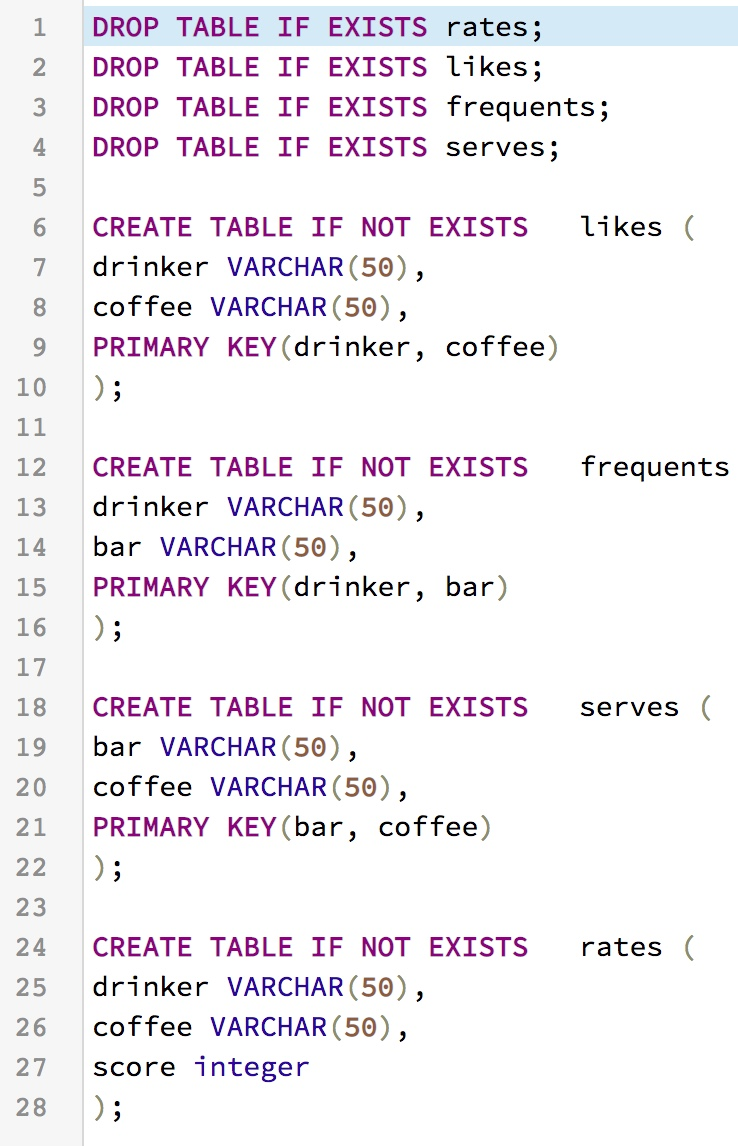
\includegraphics[width=0.7\textwidth]{./lectDDL/replay.jpg}\par}
\end{column}
\end{columns}

\end{frame}
%***********************************************************
\begin{frame}{\texttt{ALTER TABLE}}

\begin{enumerate}
\item Add / delete columns
\item Rename table / columns
\item Add / delete constraints
\item Change column data type
\begin{itemize}
\item Some systems import everything as characters
\item This can be a best practice: import as text, convert to ``correct'' data type
\end{itemize}
\item Change keys
\item Typically, CANNOT change attribute order
\end{enumerate}

\begin{itemize}
\item[?] Why import data as text?
\item[?] When might you change a key?
\end{itemize}
% you have no idea what's in the table - this way you can load it all
% you have learned more about your data, or want to store additional information in a table. E.g. add Year attribute to table and key
\end{frame}

%***********************************************************
\begin{frame}{\texttt{ALTER TABLE}}

When might you alter a table?
\begin{itemize}
\item When there is additional data to store
\item When you need to differentiate data
\item When you learn something new about the data
\item When you have to correct for defaults (Load data in SQL Server)
\item When you want to disambiguate a column or table name
\item  $\ldots$
\end{itemize}
\end{frame}

%***********************************************************
\begin{frame}{Populating Tables}

\begin{itemize}
\item \texttt{INSERT} statements
\item Product specific load/copy statements
\item GUI tools
\end{itemize}
\end{frame}

%***********************************************************
\begin{frame}[fragile]{\texttt{INSERT INTO} by Constant Value}

\begin{SQL}
INSERT INTO <tableName> [(columnName [, columnName] $\ldots$)] 
	VALUES (valueList) [, (valueList)]$\ldots$;
\end{SQL}

\end{frame}

%***********************************************************
\begin{frame}[fragile]{\texttt{INSERT INTO} by Constant Value Example}

ROOM(\underline{classroomId}, building, abbrev, room)

\begin{SQL}
INSERT INTO Room (classroomId, building, abbrev, room) VALUES
   ('DCH1070','Duncan Hall', 'DCH', '1070'),
   ('DCH1055','Duncan Hall', 'DCH', '1055'),
   ('HRZ211','Herzstein Hall', 'HRZ', '211'),
   ('SEW305','Sewell Hall', 'SEW', '305');
\end{SQL}

\end{frame}


%***********************************************************
\begin{frame}[fragile]{\texttt{INSERT INTO} by Constant Value Example}

ROOM(\underline{classroomId}, building, abbrev, room)

\begin{SQL}
INSERT INTO Room (classroomId, building, room) VALUES
   ('DCH1070','Duncan Hall', '1070'),
   ('DCH1055','Duncan Hall', '1055'),
   ('HRZ211','Herzstein Hall',  '211'),
   ('SEW305','Sewell Hall',  '305');
\end{SQL}

\begin{itemize}
\item[?] What goes into the abbrev field?
\end{itemize}
% nulls

\end{frame}

%***********************************************************
\begin{frame}[fragile]{\texttt{INSERT INTO} by Query}

\begin{SQL}
INSERT INTO <tableName> [(columnName [, columnName] $\ldots$)] 
	<SELECT statement>;
\end{SQL}

\end{frame}
%***********************************************************
\begin{frame}[fragile]{\texttt{INSERT INTO} by Query Example}

MEMBER (\underline{memberId}, lastName, firstName, memberType, startDate)
STUDENT(\underline{NETID}, FIRSTNAME, LASTNAME)\\

\begin{SQL}
INSERT INTO Member (memberId, lastname, firstName, memberType)
	SELECT netId, lastName, firstName, 'Student' 
	FROM Student;
\end{SQL}


\end{frame}
%***********************************************************
\begin{frame}[fragile]{\texttt{INSERT INTO} by Query Example 2}

MEMBER (\underline{memberId}, lastName, firstName, memberType, startDate)
STUDENT(\underline{NETID}, FIRSTNAME, LASTNAME)\\

\begin{SQL}
INSERT INTO Member (memberId, lastName, firstName, memberType)
	SELECT netId, lastName, firstName, 'Student' 
	FROM Student
	WHERE netId NOT IN 
		(SELECT memberId FROM Member);
\end{SQL}

\begin{itemize}
\item[?] What does this query do?
\end{itemize}
% Here we are inserting values into Member based on what is NOT already in the table
%So, if rbm2 were already in as faculty, she would not be inserted as a student

\end{frame}

%***********************************************************
\begin{frame}{\texttt{INSERT INTO} Notes}

\begin{itemize}
\item The entire query is evaluated before any tuples are inserted - this is why the statement on the last slide works
\item The entire operation fails if just one value cannot be inserted
\begin{itemize}
\item[?] When might this happen? % when a type is off (illegal char)
\end{itemize}
\item All constraints are checked

\end{itemize}
\end{frame}

%***********************************************************
\begin{frame}{Populating Tables in Bulk}

\begin{itemize}
\item Every RDBMS has some variant of this functionality
\begin{itemize}
\item \texttt{LOAD} in MySQL
\item \texttt{COPY} in postgres
\end{itemize}
\item Faster and more space efficient than \texttt{INSERT INTO} commands
\item You specify
\begin{itemize}
\item File name and location (path)
\item Delimiter
\item Header / no header
\item $\dots$
\end{itemize}
\end{itemize}

\end{frame}

%***********************************************************
\begin{frame}[fragile]{\texttt{DELETE}}

\begin{SQL}
DELETE FROM <tableName>
   [WHERE where_clause]
\end{SQL}

\begin{itemize}
\item Deletes records from <tableName> that meet the specified criteria
\item Reports how many rows were deleted
\item Is slower than \texttt{TRUNCATE TABLE}
\item Executes delete trigger(s)
\end{itemize}
\end{frame}

%***********************************************************
\begin{frame}[fragile]{\texttt{DELETE} Example}

ENROLL(\underline{NETID}, \underline{CRN})\\
\begin{SQL}
DELETE FROM Enroll
WHERE netId = 'abc1' AND crn = 12345;
\end{SQL}
\vspace{2em}
\begin{columns}[T]
\begin{column}{0.3\textwidth}
\begin{tabular}{|l|l|} \hline
\textbf{netId} & \textbf{crn} \\ \hline
abc1 & 12345 \\ \hline
abc1 & 34567 \\ \hline
xyz5 & 12345 \\ \hline
hj9 & 89394 \\ \hline
\end{tabular}
\end{column}
\begin{column}{0.3\textwidth}
BECOMES
\end{column}
\begin{column}{0.3\textwidth}
\begin{tabular}{|l|l|} \hline
\textbf{netId} & \textbf{crn} \\ \hline
\rowcolor{black}abc1 & 12345 \\ \hline
abc1 & 34567 \\ \hline
xyz5 & 12345 \\ \hline
hj9 & 89394 \\ \hline
\end{tabular}
\end{column}
\end{columns}

\end{frame}

%***********************************************************
\begin{frame}[fragile]{\texttt{DELETE} Implementation Details}

Usually implemented in 2 passes
\begin{enumerate}
\item Marks all candidate rows that meet the WHERE condition
\begin{enumerate}
\item Checks for constraints
\item Entire contents of table is available 
\end{enumerate}
\item Deletes the marked rows
\begin{enumerate}
\item Then updates indexes, etc.
\end{enumerate}
\end{enumerate}

\end{frame}
%***********************************************************
\begin{frame}[fragile]{\texttt{DELETE} Based on Data in Another Table}

COURSE(\underline{CRN}, COURSENAME, SCHEDULE, STARTTIME, ENDTIME)\\

ENROLL(\underline{NETID}, \underline{CRN})\\

\begin{SQL}
DELETE 
FROM Course 
WHERE crn NOT IN 
	(SELECT crn
	 FROM Enroll);
\end{SQL}

\begin{itemize}
\item[?] What does this query do?
\end{itemize}
\end{frame}
% Deletes courses that don't have any students enrolled 

%select * 
%from student s 
%left outer join enrollment e
%on s.studentid = e.studentId;
%
%# courses with no students
%select *
%from course c
%where not exists (select * from enrollment where courseId = c.courseId)
%

%***********************************************************
\begin{frame}[fragile]{\texttt{DELETE} Based on Data in the Same Table}

COURSE(\underline{CRN}, COURSENAME, SCHEDULE, STARTTIME, ENDTIME)\\

\begin{SQL}
DELETE 
FROM Course
WHERE startTime = 
	(SELECT MIN(startTime)
	 FROM Course);
\end{SQL}

\begin{itemize}
\item[?] What does this query do?
\end{itemize}
\end{frame}
% want it to delete the course that meets earliest in the morning


%***********************************************************
%\begin{frame}[fragile]{\texttt{DELETE} Based on Data in the Same Table}
%
%COURSE(\underline{CRN}, COURSENAME, SCHEDULE, STARTTIME, ENDTIME)\\
%\begin{SQL}
%DELETE 
%FROM Course
%WHERE startTime = 
%	(SELECT MIN(startTime)
%	 FROM Course);
%\end{SQL}
%
%\begin{tikzpicture}[remember picture, overlay]
%    \node[inner sep=0pt] at (current page.center) {%
%%        \includegraphics[width=\paperwidth,height=\paperheight]{./lect10/X}%
%        \includegraphics[width=0.7\textwidth]{./lect10/X}%
%    };%
%\end{tikzpicture}
%
%\begin{itemize}
%\item What does this query do?
%\item In some RDBMSs, it works (including postgres)
%\end{itemize}
%\end{frame}
%
%
%%***********************************************************
%\begin{frame}[fragile]{\texttt{DELETE} Based on Data in the Same Table}
%
%COURSE(\underline{CRN}, COURSENAME, SCHEDULE, STARTTIME, ENDTIME)\\
%
%\begin{SQL}
%DELETE 
%FROM Course
%WHERE startTime = 
%	(SELECT earliest 
%	 FROM (SELECT MIN(startTime) earliest
%	 	FROM Course) q);
%\end{SQL}
%
%\begin{itemize}
%\item[?] What's different?
%\end{itemize}
%\end{frame}
%%Need to force the creation of a temporary table
%%MySQL doesn't let you assign an alias to a select query when it is part of any update statement.
%%Nest it in another query to separate it.
%

%***********************************************************
\begin{frame}{\texttt{DELETE} (and \texttt{UPDATE}) Workaround}

Usually implemented in 2 passes
\begin{enumerate}
\item Nest the query to force the creation of a temporary table
\end{enumerate}
or
\begin{enumerate}
\item Put the keys in a temporary table
\item Then delete / update using the list of keys
\end{enumerate}

\end{frame}

%***********************************************************
\begin{frame}[fragile]{\texttt{UPDATE}}

\begin{SQL}
UPDATE <tableName>
SET <set clause list>
[WHERE <search condition>]
\end{SQL}

\begin{itemize}
\item Updates the columns specified in the set clause list to the values specified
\end{itemize}
\end{frame}

%***********************************************************
\begin{frame}[fragile]{\texttt{UPDATE} Example 1}

STUDENT(\underline{NETID}, FIRSTNAME, LASTNAME, GPA)\\
\vspace{2em}
Reset the GPA of all students
\vspace{2em}

\begin{SQL}
UPDATE Student
   SET GPA = NULL;
\end{SQL}


\end{frame}

%***********************************************************
\begin{frame}[fragile]{\texttt{UPDATE} Example 2}

COURSE(\underline{CRN}, COURSENAME, SCHEDULE, STARTTIME, ENDTIME)\\
STUDENT(\underline{NETID}, FIRSTNAME, LASTNAME, GPA)\\
ENROLL(\underline{NETID}, \underline{CRN})\\
\vspace{2em}
\begin{itemize}
\item[?] Set the GPA of all students enrolled in COMP 430 or COMP 533 to 4.0
\end{itemize}
\end{frame}

%***********************************************************
\begin{frame}[fragile]{\texttt{UPDATE} Example 2}

COURSE(\underline{CRN}, COURSENAME, SCHEDULE, STARTTIME, ENDTIME)\\
STUDENT(\underline{NETID}, FIRSTNAME, LASTNAME, GPA)\\
ENROLL(\underline{NETID}, \underline{CRN})\\
\vspace{2em}
\begin{noindentitemize}
\item Set the GPA of all students enrolled in COMP 430 or COMP 533 to 4.0
\end{noindentitemize}

\begin{SQL}
UPDATE Student 
	SET GPA = 4.0 
	WHERE netId IN 
		(SELECT netId 
		 FROM Enroll e, Course C 
		 WHERE e.crn = c.crn
			AND courseName IN ('COMP 533', 'COMP 430'));

\end{SQL}

\end{frame}

%***********************************************************
\begin{frame}[fragile]{\texttt{UPDATE} Example 3}

STUDENT(\underline{NETID}, FIRSTNAME, LASTNAME, GPA)\\
GRADE(\underline{NETID}, \underline{CRN}, \underline{ASSIGNMENT}, \underline{GRADE})\\
\vspace{2em}
\begin{noindentitemize}
\item[?] Set the GPA of all the students based on the average of their grades
\end{noindentitemize}

\begin{SQL}
UPDATE Student 
SET gpa = (?);
\end{SQL}

\end{frame}


%***********************************************************
\begin{frame}[fragile]{\texttt{UPDATE} Example 3}

STUDENT(\underline{NETID}, FIRSTNAME, LASTNAME, GPA)\\
GRADE(\underline{NETID}, \underline{CRN}, \underline{ASSIGNMENT}, \underline{GRADE})\\
\vspace{2em}
\begin{noindentitemize}
\item Set the GPA of all the students based on the average of their grades
\end{noindentitemize}

\begin{SQL}
UPDATE Student 
SET gpa = (SELECT ROUND(AVG(g.grade),2)
           FROM Grade g
           WHERE g.netId = student.netId
           GROUP BY g.netId);
\end{SQL}

\end{frame}
	
%***********************************************************
\begin{frame}[fragile]{True/False Questions}

\begin{enumerate}
\item If there is no WHERE clause in an UPDATE statement, no rows are updated
\item Data in CSV or tab delimited format CANNOT be loaded directly into a database
\item An UPDATE could be accomplished with a DELETE followed by an INSERT.
\item If we have the relation:\\
STUDENT(\underline{NETID}, FIRSTNAME, LASTNAME, GPA)\\
Can we run: \\
\begin{SQL}
INSERT INTO STUDENT(LASTNAME, NETID) VALUES ('Myers', 'rbm2')
\end{SQL}


?

\end{enumerate}
%F : all rows are updated
%F : dbms all support some sort of bulk load function
%T 
%T P: as long as nulls are allowed for the other attributes, order can be specified by the statement
%
\end{frame}




%***********************************************************
\begin{frame}{Schemas vs. Databases}

\begin{itemize}
\item Used to describe the structure of a database
\item Often used interchangeably
\item Sometimes hierarchical
\begin{itemize}
\item A database may contain many schemas
\item Each schema has its own namespace
\end{itemize}
\end{itemize}
\end{frame}

%***********************************************************
\begin{frame}{Multiple Schemas vs. Multiple Databases}

\begin{itemize}
\item Think about permissions
\item Think about size
\item Think about backups
\item Consult your Database Administrator!
\end{itemize}
\end{frame}


%***********************************************************


\begin{frame}{Wrap up}
\begin{itemize}
	\item[?] How can we use what we learned today?
	\vspace{2em}
	\item[?] What do we know now that we didn't know before?
\end{itemize}


\end{frame}


\end{document}
